\documentclass[12pt,a4paper]{article}
\usepackage[left=2.00cm,right=2.00cm]{geometry}
\usepackage[T1]{fontenc}
\usepackage[utf8]{inputenc}
\usepackage{float}
\usepackage{caption}
\usepackage{graphicx}
\usepackage{subcaption}
\usepackage{amsmath}
\usepackage{hyperref}
\hypersetup{colorlinks=true, linkcolor=blue, urlcolor=blue,
            pdftitle={NN-Adaptive Bayesian Quantum Estimation},
            pdfauthor={Michal Chrzanowski}}
\usepackage{placeins}
\usepackage{amssymb}
\usepackage{booktabs}
\usepackage{array}
\usepackage{siunitx}
\sisetup{group-minimum-digits=4}

\graphicspath{{figures/}}
\setlength{\emergencystretch}{3em}

\title{NN-Adaptive Bayesian Quantum Estimation}
\author{Michal Chrzanowski}
\date{7 September 2026}

\begin{document}
\maketitle

% ===========================================================================
\section*{Introduction}
% ===========================================================================
This report tests reinforcement-learning algorithms that decide when to measure a qubit, so that its
frequency is learned as precisely as physically possible. The work implements adaptive Bayesian
experimental design for single-qubit Ramsey frequency estimation. A sequential Monte Carlo filter
maintains a posterior over the unknown Larmor frequency $\omega$, and a policy reads that posterior
and picks the interrogation time $t$ for the next shot. The measurement outcome then sharpens the
posterior, and the cycle repeats. The policy is trained either by reinforcement learning (TRPO) or
by a gradient-free evolutionary search (CEM), following Fiderer, Schuff \& Braun,
\emph{Neural-network heuristics for adaptive Bayesian quantum estimation}.
Two learned policies are built on one shared SMC filter and one Gymnasium environment, and are
evaluated on \num{10000} randomly selected $\omega$.
TRPO and CEM land in a statistical tie ($2.173\times10^{-3}$ vs $2.137\times10^{-3}$ Bayes risk).

\begin{table}[H]
  \centering
  \begin{tabular}{@{}>{\raggedright\arraybackslash}p{0.42\textwidth}
                    >{\raggedright\arraybackslash}p{0.42\textwidth}@{}}
    \toprule
    Full name & Abbreviation \\
    \midrule
    Sequential Monte Carlo & SMC \\
    Trust-Region Policy Optimisation & TRPO \\
    Cross-Entropy Method & CEM \\
    Effective Sample Size & ESS \\
    Reinforcement Learning & RL \\
    \bottomrule
  \end{tabular}
\end{table}

\noindent\rule{\textwidth}{0.4pt}
\FloatBarrier

% ===========================================================================
\section*{Table of contents}
% ===========================================================================
\begin{itemize}
  \item \hyperref[sec:the-experiment]{The experiment}
  \item \hyperref[sec:the-physics]{The physics}
  \item \hyperref[sec:configuration]{Parameters}
  \item \hyperref[sec:the-methods]{The methods: TRPO and CEM}
  \item \hyperref[sec:training]{Training}
  \item \hyperref[sec:evaluation]{Evaluation}
  \item \hyperref[sec:analysis-of-output-data]{Analysis of output data}
  \item \hyperref[sec:summary]{Summary}
  \item \hyperref[sec:literature]{Literature}
\end{itemize}

\noindent\rule{\textwidth}{0.4pt}
\FloatBarrier

% ===========================================================================
\section{The experiment}
\label{sec:the-experiment}
% ===========================================================================
The system is a single qubit undergoing Ramsey interferometry in the presence of pure dephasing:

\begin{enumerate}
  \item Prepare $|+\rangle = (|0\rangle + |1\rangle)/\sqrt{2}$.
  \item Let it precess freely under $H = \tfrac{\omega}{2}\sigma_z$ for a time $t$. This is the
  control variable - the one thing the experimenter chooses.
  \item Apply a $\pi/2$ read-out pulse and measure in the computational basis.
  \item Record the binary outcome $d \in \{0, 1\}$.
\end{enumerate}
The qubit is not isolated: transverse noise destroys the coherence $\rho_{01}(t) =
\rho_{01}(0)\,e^{-t/T_2}e^{-i\omega t}$ on a timescale $T_2$.

\noindent\rule{\textwidth}{0.4pt}
\FloatBarrier

% ===========================================================================
\section{The physics}
\label{sec:the-physics}
% ===========================================================================

% ---------------------------------------------------------------------------
\subsection{The likelihood}
\label{sec:the-likelihood}
% ---------------------------------------------------------------------------
Solving the Lindblad pure-dephasing master equation and applying the Born rule gives the outcome
probability

\begin{align}
P(d=0 \mid \omega, t)
  &= e^{-t/T_2}\cos^{2}\!\left(\frac{\omega t}{2}\right) + \frac{1 - e^{-t/T_2}}{2} \nonumber \\
  &\equiv \frac{1}{2}\bigl[\, 1 + e^{-t/T_2}\cos(\omega t) \,\bigr],
\label{eq:likelihood}
\end{align}
and $P(d=1) = 1 - P(d=0)$. The two forms are algebraically identical.

The expression reads as a decaying interference fringe:

\begin{table}[H]
  \centering
  \caption{The likelihood.}
  \label{tab:the-likelihood}
  \small
  \begin{tabular}{ll}
  \toprule
  term & meaning \\
  \midrule
  $\cos^2(\omega t/2)$ & the Ramsey fringe - this is what carries information about $\omega$ \\
  $v(t) = e^{-t/T_2}$ & the visibility, or coherent fraction \\
  $(1-v)/2$ & the fully dephased fraction, which returns a coin flip and tells you nothing \\
  \bottomrule
  \end{tabular}
\end{table}
As $t \to \infty$ the visibility vanishes, $P(d=0) \to 1/2$, and the measurement becomes pure noise.
Decoherence therefore imposes a hard ceiling on how long it is worth interrogating.

Both the simulator and the filter's likelihood use this same expression, and $T_2$ is treated as
exactly known. The model is well-specified: there is no model mismatch and no nuisance parameter.


% ---------------------------------------------------------------------------
\subsection{The competing constraint: phase ambiguity}
\label{sec:the-competing-constraint-phase-ambiguity}
% ---------------------------------------------------------------------------
Fisher information is a \emph{local} quantity, and maximising it is the wrong move while the prior
is still broad. The likelihood depends on $\omega$ only through $\cos(\omega t)$, which is periodic.
Over the prior support $\Delta\omega = 1$ the fringe wraps once $t > 2\pi \approx 6.28$: several
well-separated $\omega$ then produce the same phase. The posterior goes multimodal, and the filter
cannot resolve the aliases.

A good policy must therefore trade off:

\begin{itemize}
  \item small $t$ - unambiguous, but low information per shot ($I \sim t^2$).
  \item $t \approx T_2$ - maximum information per shot, but aliases a broad prior.
  \item $t \gg T_2$ - decohered, zero information, strictly wasted.
\end{itemize}
The resolution is to grow $t$ \emph{as the posterior narrows}, so the phase spread stays near one
radian. A learned policy is expected to discover this.

% ---------------------------------------------------------------------------
\subsection{The figure of merit: Bayes risk}
\label{sec:the-figure-of-merit-bayes-risk}
% ---------------------------------------------------------------------------
This is a Bayesian estimation problem, and the quantity everything is judged by is the Bayes risk -
Fiderer Eq. (1):

\begin{equation}
r\bigl(h \mid p(\theta)\bigr) = \mathbb{E}_{D_k}\bigl[\, \mathrm{tr}\,\mathrm{Cov}(\theta \mid D_k)
\,\bigr],
\label{eq:bayes-risk}
\end{equation}
where $h$ is the experiment-design heuristic, $D_k = (d_1,\dots,d_k)$ the measurement record, and
smaller is better. It is the risk of the quadratic loss $L(\hat\theta_k, \theta) =
\lVert\hat\theta_k - \theta\rVert_2^2$ under the Bayes estimator $\hat\theta_k(D_k) =
\mathbb{E}[\theta \mid D_k]$. That is, the posterior mean, which is exactly what this implementation
reports as \texttt{posterior\_\allowbreak{}mean}.

Here the trace is over a $1\times1$ covariance, and the expectation is averaged over true $\omega$
values. So the Bayes risk is precisely the mean final posterior variance reported as
\texttt{final\_\allowbreak{}variance\_\allowbreak{}mean}. They are the same number. The paper's name
for it is the Bayes risk.

The paper is explicit that the \emph{frequentist} route goes ``with the Cram\'er-Rao bound formalism
by maximizing the quantum Fisher information''. It
deliberately takes the Bayesian route instead. Fisher information is a useful sanity check here
(\hyperref[sec:aside-why-long-interrogation-times-stop-helping]{above}) but it is not the objective.

% ---------------------------------------------------------------------------
\subsection{The reward}
\label{sec:the-reward}
% ---------------------------------------------------------------------------
The reward is the reduction in traced posterior covariance at each step - Fiderer Eq. (2):

\begin{align}
R(D_k) &= \mathrm{tr}\,\mathrm{Cov}(\theta \mid D_{k-1}) - \mathrm{tr}\,\mathrm{Cov}(\theta \mid
D_k) \nonumber \\
       &\xrightarrow{\ d=1\ } V_{k-1} - V_k,
\label{eq:reward}
\end{align}
with $V_k = \sum_i w_i(\omega_i - \bar\omega)^2$. This is not an arbitrary choice, and it is not a
weaker substitute for an information-gain reward. The paper's reasoning: the negative Bayes risk is
the obvious reward but is far too slow to compute inside a training loop. Eq. (2) is cheap in the
SMC framework \emph{and} telescopes to it. Eq. (3), for $N$ experiments per episode:

\begin{equation}
\mathbb{E}_{D_N}\left[\sum_{j=1}^{N} R(D_j)\right] = \mathrm{const} - r\bigl(h \mid p(\theta)\bigr),
\qquad \mathrm{const} = \mathrm{tr}\,\mathrm{Cov}(\theta).
\label{eq:telescope}
\end{equation}
So maximising the episode return provably minimises the Bayes risk, provided the return is
undiscounted ($\gamma = 1$).

\noindent\rule{\textwidth}{0.4pt}
\FloatBarrier

% ===========================================================================
\section{Parameters}
\label{sec:configuration}
% ===========================================================================
A single shared parameter set backs every comparison.

\begin{table}[H]
  \centering
  \caption{What is being estimated.}
  \label{tab:what-is-being-estimated}
  \footnotesize
  \begin{tabular}{%
    >{\raggedright\arraybackslash}p{0.124\linewidth}%
    >{\raggedright\arraybackslash}p{0.782\linewidth}}
  \toprule
  quantity & value \\
  \midrule
  parameter & $\omega$, a single scalar (the Larmor frequency / detuning) \\
  prior & $\omega \sim \mathrm{Uniform}(0, 1)$ \\
  true values & drawn from the same $\mathrm{Uniform}(0,1)$ \\
  coherence time & $T_2 = 10$ \\
  control & $t \in [0.1,\ 3000]$ \\
  particles & $10^4$ train / $2\times10^3$ eval \\
  episode & 100 measurements (training) / 125 (evaluation) \\
  reference evaluation & \num{10000} $\omega$ \\
  \bottomrule
  \end{tabular}
\end{table}

\noindent\rule{\textwidth}{0.4pt}
\FloatBarrier

% ===========================================================================
\section{The methods: TRPO and CEM}
\label{sec:the-methods}
% ===========================================================================

% ---------------------------------------------------------------------------
\subsection{The inference layer: SMC particle filter}
\label{sec:the-inference-layer-smc-particle-filter}
% ---------------------------------------------------------------------------
$\omega$ is a static parameter that does not evolve, so the filter only ever reweights particles.
The particle locations move only during resampling.

Representation. $N$ particles $\{\omega_i\}$ with log-weights $\{\log w_i\}$. Shapes are \texttt{(N,
1)} / \texttt{(N,)} in the NumPy path, \texttt{(B, N, 1)} / \texttt{(B, N)} in the batched Torch
path, where \texttt{B} indexes independent experiments.

Bayes update. Log-domain throughout:

\begin{equation}
\log w_i \leftarrow \log w_i + \log P(d \mid \omega_i, t) - \mathrm{logsumexp}(\cdot).
\label{eq:bayes-update}
\end{equation}
Renormalised every step, so weights always sum to one.

Effective sample size. The Kish ESS, $\mathrm{ESS} = 1/\sum_i w_i^2 \in [1, N]$.

Resampling fires when $\mathrm{ESS} < 0.75N$, an aggressive threshold (0.5N is the usual default),
so it triggers on most steps. Two schemes exist, but the default everywhere is Liu-West kernel
resampling ($a = 0.98$):

\begin{equation}
\omega_i' = a\,\omega_{\mathrm{idx}(i)} + (1-a)\,\bar{\omega} + \varepsilon_i,
\qquad \varepsilon_i \sim \mathcal{N}\bigl(0,\, h^{2}\Sigma\bigr), \quad h^{2} = 1 - a^{2}.
\label{eq:liu-west}
\end{equation}
The shrinkage toward the weighted mean exactly cancels the variance added by the jitter ($a^2\Sigma
+ h^2\Sigma = \Sigma$), so the posterior's first two moments are preserved. The jitter is what
prevents particle impoverishment. Plain multinomial resampling would collapse all particles onto a
handful of duplicated values, since a static parameter never gets diffused by process noise.

% ---------------------------------------------------------------------------
\subsection{The control problem}
\label{sec:the-control-problem}
% ---------------------------------------------------------------------------
The control problem is framed as a Gymnasium environment, \texttt{AdaptiveSMCEnv}:

\begin{table}[H]
  \centering
  \caption{The control problem.}
  \label{tab:the-control-problem}
  \scriptsize
  \begin{tabular}{ll}
  \toprule
  observation & \texttt{[posterior\_\allowbreak{}mean, posterior\_\allowbreak{}var,
  *last\_\allowbreak{}30\_\allowbreak{}interrogation\_\allowbreak{}times]} $\rightarrow$
  \texttt{Box(32,)} \\
  action & interrogation time $t$ $\rightarrow$ \texttt{Box(0.\allowbreak{}1, 3000.\allowbreak{}0,
  (1,))} \\
  reward & $V_{k-1} - V_k$ \\
  episode & 100 measurements (training) / 125 (evaluation), one true $\omega$ per episode \\
  \bottomrule
  \end{tabular}
\end{table}

% ---------------------------------------------------------------------------
\subsection{The two learned policies}
\label{sec:family-learned}
% ---------------------------------------------------------------------------
Two learned policies are implemented:

\begin{table}[H]
  \centering
  \caption{Learned policies.}
  \label{tab:learned-policies}
  \footnotesize
  \begin{tabular}{%
    >{\raggedright\arraybackslash}p{0.09\linewidth}%
    >{\raggedright\arraybackslash}p{0.257\linewidth}%
    >{\raggedright\arraybackslash}p{0.357\linewidth}}
  \toprule
  method & optimiser & network \\
  \midrule
  TRPO & trust-region policy optimisation (\texttt{sb3\_\allowbreak{}contrib}) & \texttt{MlpPolicy},
  $\pi$ and $V$ both \texttt{[256, 256]} \\
  CEM & cross-entropy method over the flat 545-dim weight vector &
  \texttt{TimePolicy\_\allowbreak{}Fiderer\_\allowbreak{}16} - one hidden layer of 16,
  \texttt{Tanh}, sigmoid-squashed output \\
  \bottomrule
  \end{tabular}
\end{table}
The CEM network squashes its output structurally, $t = t_{\min} + (t_{\max}-t_{\min})\,\sigma(z)$,
so it can never emit an out-of-range time. The TRPO actor is an unbounded Gaussian whose sample is
clipped in the environment step.

\subsubsection{1. TRPO}
\label{sec:method-trpo}
Reads \texttt{[posterior\_\allowbreak{}mean, posterior\_\allowbreak{}var,
*last\_\allowbreak{}30\_\allowbreak{}interrogation\_\allowbreak{}times]} $\rightarrow$
\texttt{Box(32,)} and emits an unbounded Gaussian sample of $t$, clipped to $[0.1, 3000]$ in the
environment step. The $\pi$ and $V$ heads are both \texttt{[256, 256]} MlpPolicy. The optimiser is
the trust-region policy optimiser from \texttt{sb3\_\allowbreak{}contrib} with
\texttt{target\_\allowbreak{}kl} $= 10^{-2}$ and $\gamma = 0.99$. TRPO is trained from scratch for
$10^7$ timesteps.

Training is the standard trust-region loop, one update per rollout batch:

\begin{enumerate}
  \item Collect experience. The agent plays episodes in \texttt{AdaptiveSMCEnv}. Each episode draws
  one true frequency, runs \num{100} measurements, observes \texttt{[posterior mean, posterior
  variance, last 30 interrogation times]} and receives the reward $V_{k-1} - V_k$. \num{2048}
  environment steps are gathered per update - the \texttt{sb3\_\allowbreak{}contrib} default, left
  unoverridden here.
  \item Estimate advantages. Generalised advantage estimation with $\gamma = 0.99$ and $\lambda =
  0.95$ converts the reward sequence into a normalised advantage $\hat A$ for every step, using the
  value head as the baseline.
  \item Fit the value function. The critic takes \num{10} gradient steps per update, which lowers
  the variance of $\hat A$.
  \item Take a trust-region step. The actor maximises the surrogate
  $\mathbb{E}\!\left[\frac{\pi_\theta(a\mid s)}{\pi_{\theta_{\mathrm{old}}}(a\mid s)}\,\hat
  A\right]$ subject to $\mathbb{E}\!\left[D_{\mathrm{KL}}(\pi_{\theta_{\mathrm{old}}} \,\|\,
  \pi_\theta)\right] \le 10^{-2}$. The search direction is the natural gradient, obtained by
  conjugate gradients (at most \num{15} iterations, damping $0.1$). A backtracking line search then
  shrinks the step by $0.8$ until the KL constraint holds and the surrogate improves. If no such
  step exists, the update is reverted.
  \item Repeat. Steps 1-4 run for $10^5$ episodes ($10^7$ timesteps). The shipped policy is the
  network after the last update.
\end{enumerate}

\subsubsection{2. CEM}
\label{sec:method-cem}
A gradient-free cross-entropy method over the flat 545-dim weight vector of
\texttt{TimePolicy\_\allowbreak{}Fiderer\_\allowbreak{}16} - one hidden layer of 16, \texttt{Tanh},
sigmoid-squashed output. Population 1000, elite fraction 0.1,
\texttt{CEM\_\allowbreak{}INIT\_\allowbreak{}STD = 1.\allowbreak{}0}, with 100-step episodes and 2000
particles.

Training is a generation loop over that weight vector:

\begin{enumerate}
  \item Initialise the search distribution. The network's parameters are flattened into a
  \num{545}-dimensional vector $\theta$, and the search starts from $\mu = 0$ and $\sigma = 1.0$.
  \item Sample a population. Draw \num{1000} candidates $\theta_i \sim \mathcal{N}(\mu, \sigma^2)$.
  \item Score each candidate. Each $\theta_i$ is copied into the network, which maps the observation
  through \num{16} \texttt{Tanh} units and squashes its output with a sigmoid, $t = t_{\min} +
  (t_{\max} - t_{\min})\,\sigma(z)$. The candidate's return is the total reward of one full episode
  played at that generation's true frequency.
  \item Select the elite. Rank the \num{1000} candidates by return and keep the best \num{100}
  (elite fraction $0.1$).
  \item Refit the distribution. Set $\mu$ to the elite mean and $\sigma$ to the elite standard
  deviation, so the next generation samples around the better parameters.
  \item Repeat. Steps 2-5 run for \num{100} generations. The returned policy is the final $\mu$,
  not a sampled population member.
\end{enumerate}

\noindent\rule{\textwidth}{0.4pt}
\FloatBarrier

% ===========================================================================
\section{Training}
\label{sec:training}
% ===========================================================================
TRPO. Training runs for $10^5$ episodes of 100 steps, or $10^7$ timesteps, with \num{10000}
particles, \texttt{[256, 256]} policy and value networks, and \texttt{target\_\allowbreak{}kl}
$= 10^{-2}$. Checkpoints are written every \num{50000} timesteps. A partially trained policy can
then be evaluated at any point, and a crash costs at most one interval.

TRPO is trained from scratch.

CEM. Training runs for 100 generations at population 1000, elite fraction 0.1, with 2000 particles
and 100-step episodes, optimising the flat 545-dimensional weight vector of
\texttt{TimePolicy\_\allowbreak{}Fiderer\_\allowbreak{}16}. This takes about 45 minutes on CPU,
roughly 27\,s per generation.

Logging. Logged per episode (TRPO) or per generation (CEM): \texttt{mean\_\allowbreak{}reward},
\texttt{mean\_\allowbreak{}init\_\allowbreak{}var},
\texttt{mean\_\allowbreak{}final\_\allowbreak{}var}, \texttt{mean\_\allowbreak{}ess},
\texttt{mean\_\allowbreak{}t}, \texttt{true\_\allowbreak{}omega}. Plus
\texttt{max\_\allowbreak{}reward}, \texttt{sigma\_\allowbreak{}mean} and
\texttt{mu\_\allowbreak{}norm} for CEM. Parameters capture the full hyperparameter set.

\noindent\rule{\textwidth}{0.4pt}
\FloatBarrier

% ===========================================================================
\section{Evaluation}
\label{sec:evaluation}
% ===========================================================================
Both policies are scored through one shared NumPy reference harness, which runs at float64 and
follows one true frequency at a time. The harness is method-agnostic. The SMC filter, the
measurement model and the scoring code are identical for TRPO and CEM. The only method-specific part
is the function that maps the posterior summary to the next interrogation time $t$. The procedure
below is therefore the evaluation of both policies.

\begin{enumerate}
  \item Draw the test frequencies. Draw $N$ true frequencies $\omega \sim \mathrm{Uniform}(0,1)$
  from a fixed seed. The draw is independent of the training draw, so these are genuinely held-out
  frequencies.
  \item Initialise the filter. Represent the prior by \num{2000} particles drawn
  $\mathrm{Uniform}(0,1)$ with uniform weights. This is the belief before the first measurement.
  \item Run one episode. Repeat the following \num{125} times, once per measurement:
  \begin{enumerate}
    \item Read the belief. Normalise the particle weights, compute the posterior mean and variance
    from them. Assemble the observation the policy sees: the mean, the variance, then the last
    \num{30} chosen interrogation times (all zero before the first step).
    \item Choose the interrogation time. The policy maps that observation to a single $t$, clipped
    to $[0.1, 3000]$.
    \item Simulate the measurement. Draw the binary outcome $d \in \{0,1\}$ from $\Pr(d = 0 \mid
    \omega, t) = e^{-t/T_2}\cos^2(\omega t/2) + (1 - e^{-t/T_2})/2$ with $T_2 = 10$, evaluated at
    the \emph{true} $\omega$ of the episode.
    \item Update the posterior. Reweight every particle by the likelihood of the observed outcome
    $d$ at its own $\omega$.
    \item Resample if needed. If the effective sample size falls below $0.75 \times \num{2000} =
    \num{1500}$, resample the particles with the Liu-West scheme to restore weight diversity before
    the next step.
  \end{enumerate}
  \item Score the episode. Record that episode's final posterior variance - one number per
  frequency.
  \item Average. Average the $N$ final variances. For this single-parameter, experiment-limited
  problem the traced posterior covariance averaged over true $\omega$ is exactly the final posterior
  variance, so this average \emph{is} the Bayes risk of
  \hyperref[sec:the-figure-of-merit-bayes-risk]{Eq. (1)}. Lower is better.
\end{enumerate}

The validation reported below uses $N = \num{10000}$. The repository's general-purpose evaluator,
\texttt{pipeline/\allowbreak{}evaluate.\allowbreak{}py}, runs the same procedure over a batched
Torch rollout with \texttt{--n-omegas} defaulting to \num{2000}.

A GPU is not required. The batched rollout costs roughly 4.4\,ms per 125-step, 2000-particle episode
on CPU, so a \num{10000}-$\omega$ evaluation takes about a minute.

\noindent\rule{\textwidth}{0.4pt}
\FloatBarrier

% ===========================================================================
\section{Analysis of output data}
\label{sec:analysis-of-output-data}
% ===========================================================================

% ---------------------------------------------------------------------------
\subsection{Validation over \texorpdfstring{\num{10000}}{10 000} \texorpdfstring{$\omega$}{omega}}
\label{sec:validation-over-10-000-omega-the-n-scripts}
% ---------------------------------------------------------------------------
Both learned policies were evaluated on the NumPy reference harness over \num{10000} held-out
frequencies.

\begin{table}[H]
  \centering
  \caption{Validation over \num{10000} $\omega$ (the N-scripts).}
  \label{tab:validation-over-10-000-omega-the-n-scripts}
  \scriptsize
  \begin{tabular}{lll}
  \toprule
   & TRPO & CEM \\
  \midrule
  training & \num{100002} episodes, $10^7$ timesteps, 2 h 24 m & 99 generations $\times$ 1000 pop,
  54 min \\
  Bayes risk over \num{10000} $\omega$ & $2.173\times 10^{-3}$ & $2.137\times 10^{-3}$ \\
  mean $t$ & 4.00 & 6.67 \\
  min / max $t$ & 0.10 / 9.85 & 2.16 / 15.60 \\
  final ESS (of 2000) & 1960 & 1904 \\
  \bottomrule
  \end{tabular}
\end{table}
The two methods land in a statistical tie ($2.17\times 10^{-3}$ vs $2.14\times 10^{-3}$, a 2\%
difference) despite completely different optimisers and very different chosen times. CEM settles on
interrogation times roughly 1.7$\times$ longer than TRPO's, and never goes below $t = 2.16$, where
TRPO ranges down to the action floor.

\subsubsection{Posterior collapse}\label{sec:posterior-collapse}
Mean posterior variance across all \num{10000} $\omega$, log scale. Both fall about 1.6 decades from
the prior's 0.0833 and flatten out well before the 125th measurement - the information-starved
regime described above.

\begin{figure}[H]
  \centering
  \begin{subfigure}[t]{0.48\textwidth}
    \centering
    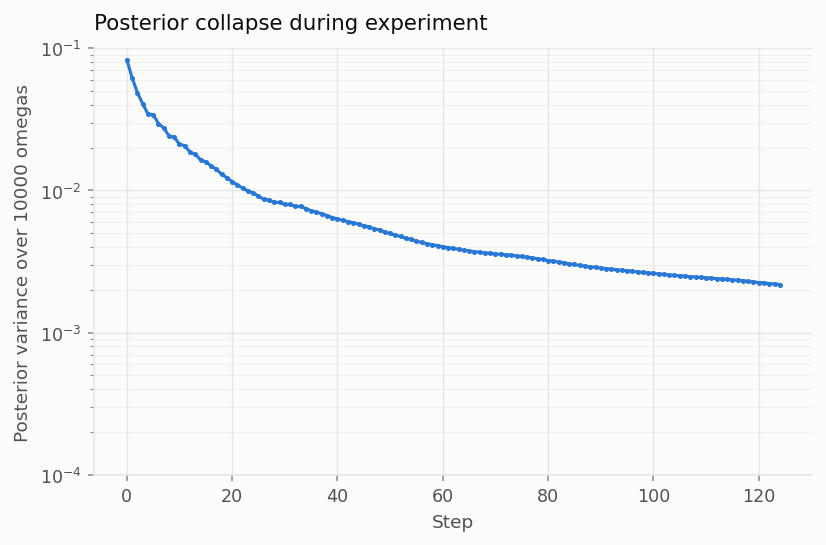
\includegraphics[width=\textwidth]{trpo_posterior_variance_over_omega_log}
    \caption{TRPO}
    \label{fig:posterior-collapse-trpo}
  \end{subfigure}\hfill
  \begin{subfigure}[t]{0.48\textwidth}
    \centering
    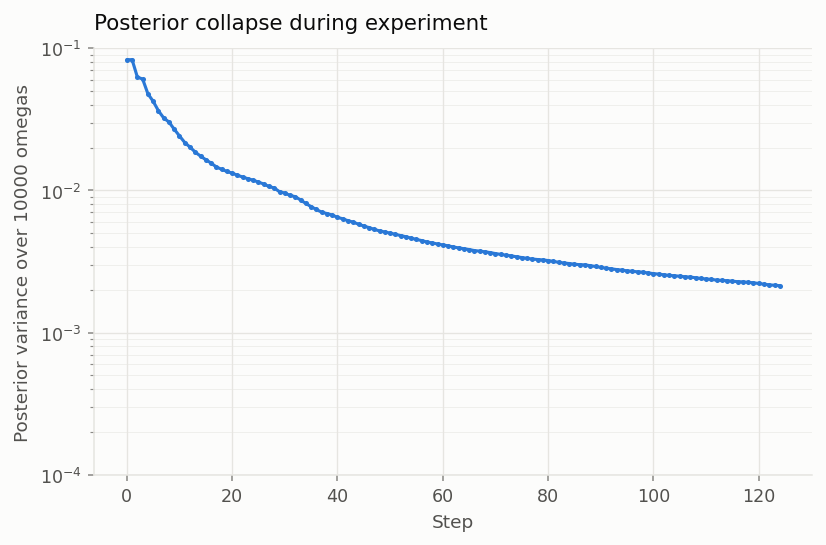
\includegraphics[width=\textwidth]{cem_posterior_variance_over_omega_log}
    \caption{CEM}
    \label{fig:posterior-collapse-cem}
  \end{subfigure}
  \caption{Posterior collapse.}
  \label{fig:posterior-collapse}
\end{figure}

\noindent\rule{\textwidth}{0.4pt}
\FloatBarrier
\section{Summary}\label{sec:summary}
The physics and the estimation machinery are in place and behave. The likelihood, the Bayes-risk
figure of merit, the variance-reduction reward and its telescoping identity all match the paper
equation by equation. The particle filter is healthy - ESS stays at $\sim$1900-1960 of 2000 and is
not the bottleneck.

Trained TRPO and CEM policies land in a statistical tie over \num{10000} held-out frequencies, at
$2.173\times10^{-3}$ and $2.137\times10^{-3}$ Bayes risk respectively. For both, the posterior
variance falls about 1.6 decades from the prior's 0.0833 and flattens out well before the 125th
measurement. CEM settles on interrogation times roughly 1.7$\times$ longer than TRPO's and never
goes below $t = 2.16$, where TRPO ranges down to the action floor. Neither policy shows the monotone
growth in $t$ that an optimal adaptive schedule should produce as the posterior narrows.

\noindent\rule{\textwidth}{0.4pt}
\FloatBarrier
\section{Literature}\label{sec:literature}
\begin{itemize}
  \item Fiderer, Schuff \& Braun, \emph{Neural-network heuristics for adaptive Bayesian quantum
  estimation}, PRX Quantum 2, 020303 (2021) - preprint dated 2020-03-05, whose equation numbers this
  report quotes.
\end{itemize}

\end{document}